\section{metoder indenfor billedbehandling}\label{subsec:kant}
Formelt kan et billede repræsenteres som en funktion af to variable:
\begin{equation}
\begin{split}
&I: \mathbb{\mathbb{Z^+}}^2 \rightarrow \mathbb{Z^+} \\
&I(x,y) = \lambda \hspace{0.5 cm} (x,y)\in \mathbb{Z^+}^2, \lambda \in [1,256] \subset \mathbb{Z^+}
\end{split}
\label{bf}
\end{equation}
hvor $\lambda$ repræsentere en billedintensitet, også kaldet pixelværdi. $\lambda$ er defineret, indenfor grænserne af billedet og er 0 udenfor, dvs.: 
\begin{equation}
 I(x, y) =
\begin{cases}
    \lambda, & \text{hvis } 1 \leq x \leq x_{max}, 1 \leq y \leq y_{max} \\
    0,              & \text{ellers}
    \label{pixelintensitet}
\end{cases}
\end{equation}
En kort bemærkning bør gøres om det anvendte billedformatet. De undersøgte billeder er af filtype JPEG(Joint Photographic Experts Group) og hver pixelintensitet indeholder originalt 8x3 bits information til hhv. rød, grøn og blå: $\lambda_{col} = [R,G,B]^T \in \mathbb{R}^3$. Hver farve kan antage $2^8 = 256$ værdier og hver værdi ligger i intervallet $[0,1]$. Disse værdier bliver transformeret til en gråtone værdi, vha. Lumosity metoden <cite>:
\begin{equation}
Lum(\lambda_{col}) = [0.2126, 0.7152, 0.0722] \lambda_{col} = \lambda
\label{lumosity}
\end{equation}
Hver gang pixelværdi eller billedintensitet benævnes, er det underforstået, at de har undergået den lineære transformation, ligning \cite{lumosity}. $x$ og/eller $y$ kan højst antage værdien 65.535, og et billede er derfor i sagens natur diskret.
\\
\\
Diskontinuitet i billeder er ofte en nyttig egenskab, i en billedanalytisk procedure. Det kan være i form af en kant: Hvis et billede beskues i 3D, kan en kant illustreres i 1D, ved et snit af et billede vinkelret på overfladen, illustreret figur \ref{fig:kant}. En kant er en lokal ændring i det afledte signal $f$.
\noindent
\begin{figure}[H]
    \centering
    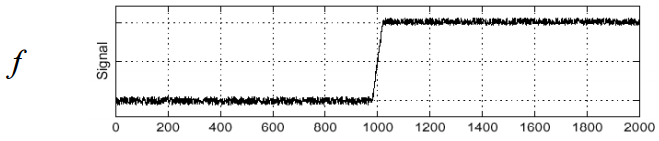
\includegraphics[width=0.55\textwidth]{fig/7.png}
     \vspace{-1em}
    \begin{center}        
     \caption{\textcolor{gray}{\footnotesize \textit{
En 1-dimensional fortolkning af intensiteten i et billede. Intensitetsskiftet i midten (ved x $approx$ 1000, er en kant.}}}
    \label{fig:kant}
     \end{center}
       \vspace{-2.5em}
  \end{figure}
\noindent
En differentiering af funktionen fra figur \ref{fig:kant} vil fremhæve dens udsving og derved angive hvor der forekommer kanter. Differentiering af billeder kan approsikmeres ved følgende ligning:
\begin{equation}
\dfrac{df(x)}{dx}=\dfrac{f(x+1)-f(x-1)}{2}
\label{diff}
\end{equation}
\\
\\
<beskriv hvorfor foldning er nyttigt>
Foldning af $I$ af størrelse $(M \times N)$, med en kerne $K$ der har størrelse $(m \times n)$, hvor $M > k, N > n$:
\begin{equation}
O(i,j) = \sum\limits_{x=1}^m \sum\limits_{y=1}^n I(i+k-1,l-1)K(k,l)
\label{foldning}
\end{equation}
Ligning \eqref{foldning} udregnes for alle $i,j \in I$. En kerne defineres her som en matrix af arbitrær dimension - ofte $(N\times N)$. 
\\
\\
Et billede kan differentieres, som anført ligning \eqref{diff}, ved brug af foldning. Først defineres en kerne til differentiering i $x$-aksen $K$, som: $K = [\frac{1}{2}, 0, \frac{1}{2}]$. Kernen foldes med billedet $I$: $I \ast K $, hvor $\ast$ udgør foldningsoperatoren.
\\
\\
Når en kerne skal foldes med et billede hvor afstanden til kanten af billedet, er skarpt mindre, end størrelsen af kernen, gælder ligning \eqref{pixelintensitet} for $I$.
\\
\\
Det kan være problematisk at lokalisere kanter vha. differentiering. I figur \ref{fig:kant}, vil støj i billedet(de små udsving) også blive fremhævede. For at fjerne støjen, kan billedet foldes med et Gaussisk filter, hvilket er en diskret approksimering til den Gaussiske funktion. Foldning af et billede med et Gaussisk filter vil resultere i en flydende overgang af pixelværdierne og derfor glatte billedet. <sæt gaussbillede ind> Den Gaussiske funktion i 2-D, hvor $ \sigma $ er standardafvigelsen af den Gaussiske fordelingen, er defineret som:
\begin{equation}
G(x,y,\sigma) = \frac{1}{2 \pi \sigma ^{2}} e^{- \frac{x^{2} + y^{2}}{2 \sigma ^{2}}}
\label{2dgaussian}
\end{equation} 
For at undgå først at glatte billedet ved at folde med et Gaussisk filter, og derefter folde med et differentieringsfilter udnyttes det, at foldning er en associativ operation:
\begin{equation}
\dfrac{\partial}{\partial x}(G \ast f) = (\dfrac{\partial}{\partial x}G) \ast f
\end{equation}
Her er $G$ er det Gaussiske filter, men kunne være en vilkårlig anden kerne, og $f$ et signal. 
\\
Foldes et differentieret 1-dimensionelt Gaussfilter med signalet fra figur \ref{fig:kant}, vil det resultere i et bakkeformet signal, hvor bakken indikere en kant. For en mere lokaliserbar kant, kan den dobbelt afledte tages, som set i figur \ref{fig:deriv}. I sidstnævnte tilfælde, kan kanten lokaliseres, hvor funktionen krydser nul.
\begin{figure}[H]
    \centering
    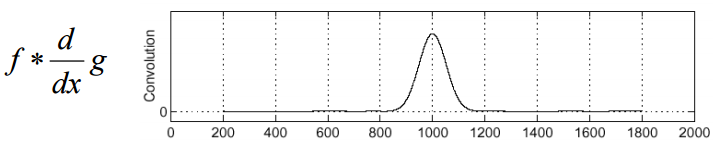
\includegraphics[width=0.55\textwidth]{fig/8.png}
    \vspace{-1em}   
    \begin{center}
    \caption{\textcolor{gray}{\footnotesize \textit{
     Resultatet af at folde et dobbelt differentieret Gaussisk filter med funktionen}}}
    \label{fig:deriv}
     \end{center}
    \vspace{-2.5em}  
  \end{figure}
\noindent
I de metoder der i denne opgave er gjort brug af, er diskontinuiteter i lokale strukturer i billederne undersøgt. Derfor er det nyttigt at bruge et dataindsamlingsvindue $\bold{D}$, da dette kan repræsentere et lokalområde. Et dataindsamlingsvindue er en $(N\times N)$ matrix over en funktion af et udsnit af et billede. For et dataindsamlingsvindue over koordinaterne $(x,y)$ tilhørende $I$ gælder, at $(x,y)$ er centrum i dataindsamlingsvinduet, dvs:
$$
\bold{D_{\frac{N}{2},\frac{N}{2}}} = f(I(x,y))
$$
de andre værdier i $\bold{D}$, er resultatet af en funktion over $I$, omkring $(x,y)$ - dette kan være identitetsfunktionen, men også være en udregning af gradienter.